\Exhibit{StackOverflowWikipedia}{%
    Статья в Wikipedia про Stack Overflow%
}

Это скриншот статьи в Wikipedia о Stack Overflow.
В ней говорится:

\begin{itemize}

    \item \Quote{Stack Overflow -- это сайт с вопросами и ответами для программистов.}

    \item \Quote{В марте 2022 на Stack Overflow было зарегистрировано больше 20 миллионов пользователей.}

    \item \Quote{Этот сайт и подобные сайты с вопросами и ответами для программистов
    в основном вытеснили книги по программированию по всему миру как источник ежедневной справочной информации в нулевых,
    и сегодня они -- важная часть программирования.}

\end{itemize}

Эти факты подтверждаеют, что опросы, проводимые Stack Overflow, авторитетны для сферы разработки ПО.

\begin{center}
    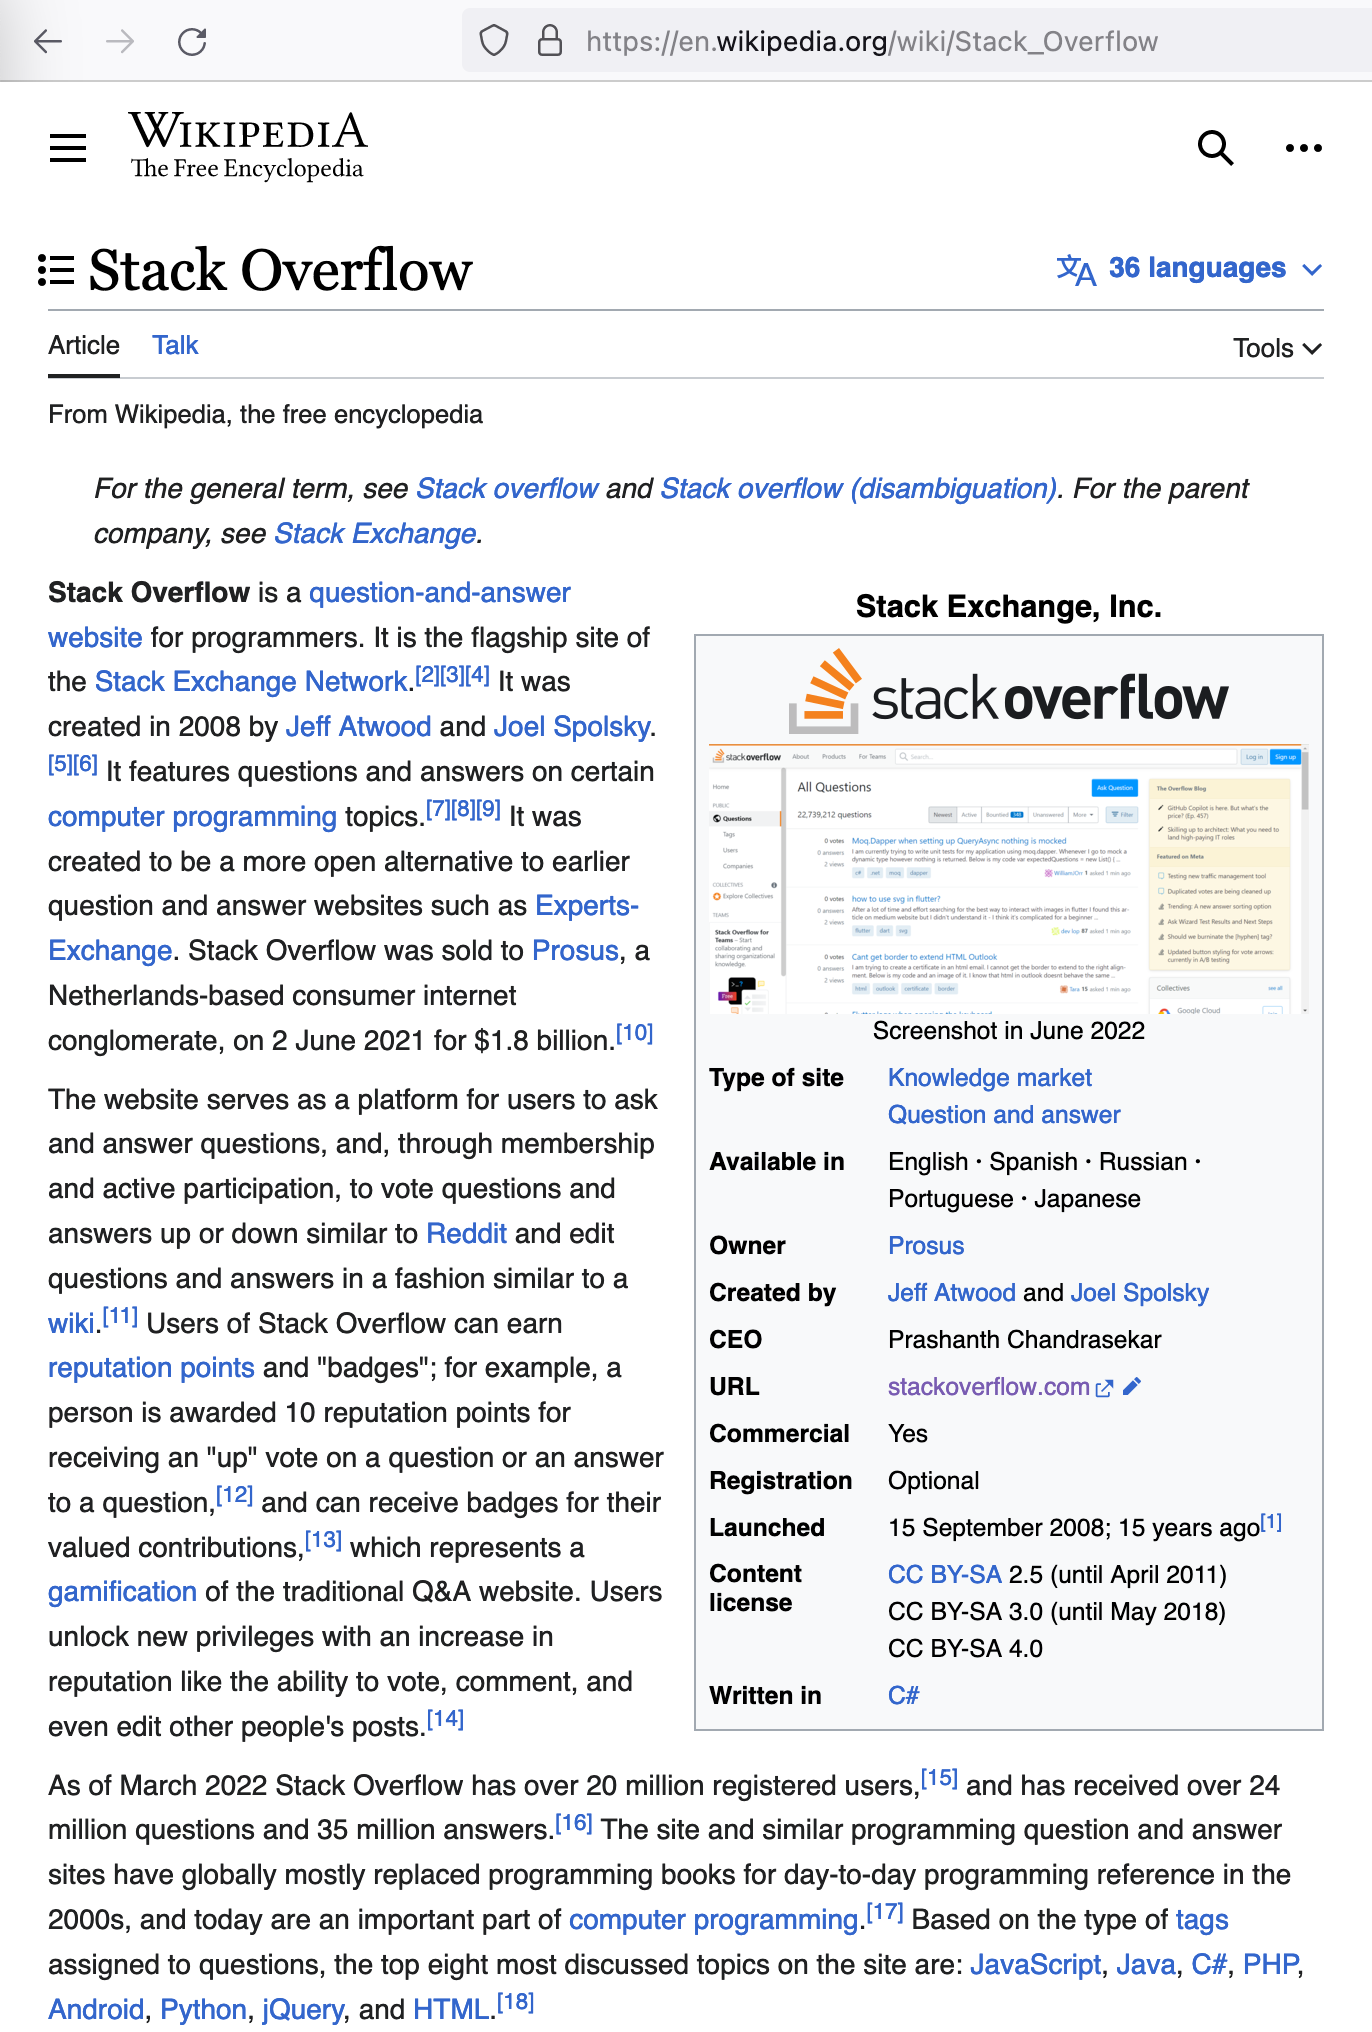
\includegraphics[width=40em]{stackoverflow-wikipedia}
\end{center}

\pagebreak
